% --- World models: motivation, definition, applications, paradigms ---
\begin{frame}{World Models: Motivation}
  \textbf{Intuition:} a baseball batter reacts in milliseconds---action is tied to a \textbf{predictive}, action-conditioned internal model, not to slow deliberate search.
  \centering
  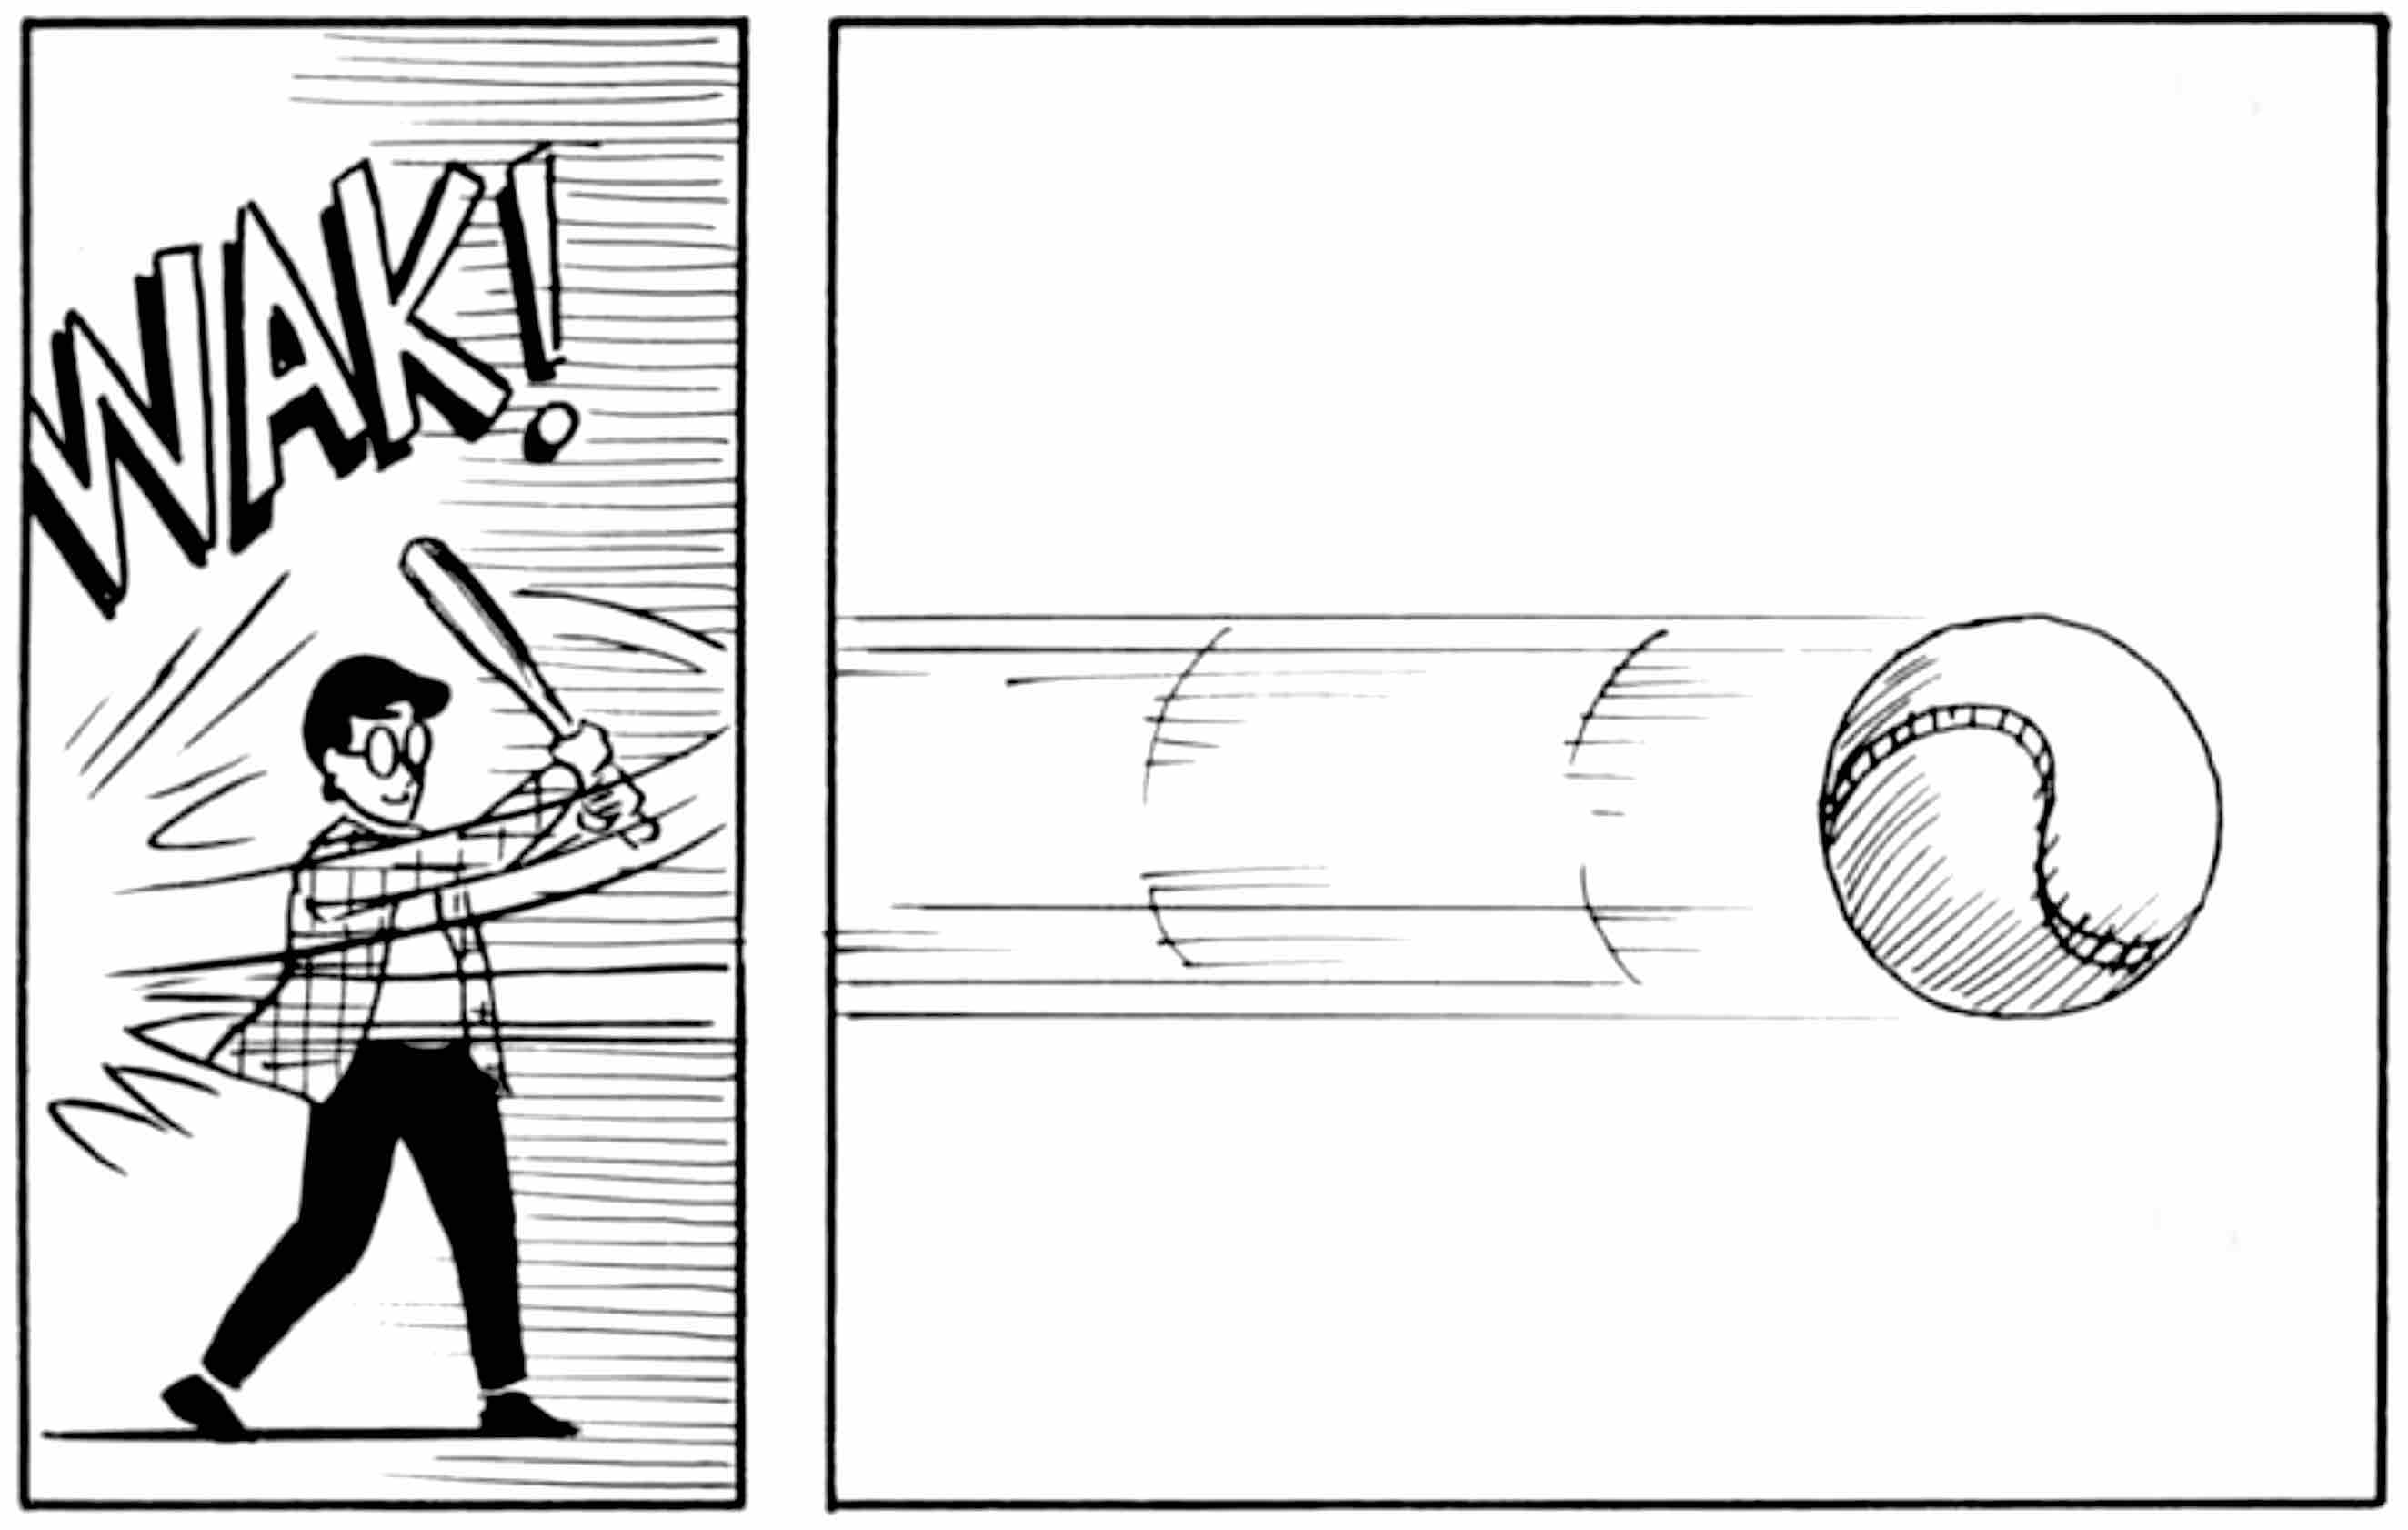
\includegraphics[width=\linewidth,height=0.72\textheight,keepaspectratio]{assets/New-Lecture_World_Models/mccloud_baseball.jpeg}\\[-0.1em]
  {\scriptsize Scott McCloud excerpt (time--space in comics).}      
\end{frame}

\begin{frame}{World Models: Motivation}
  \centering
  \vspace{0.1em}
  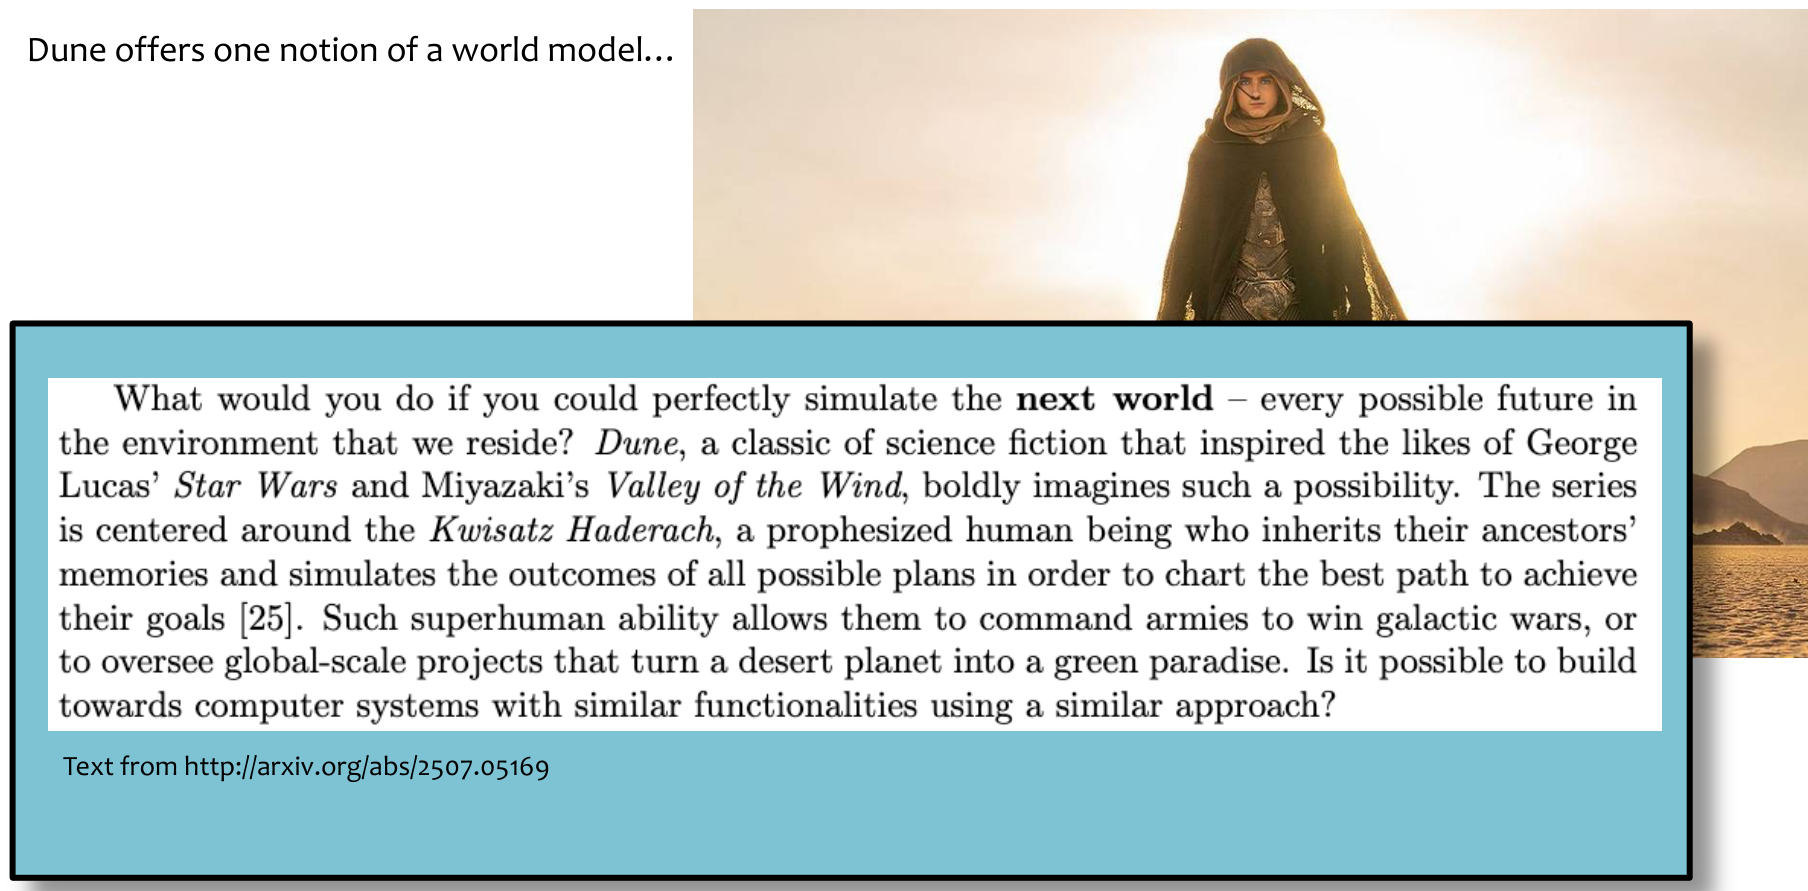
\includegraphics[width=\linewidth,height=0.88\textheight,keepaspectratio]{assets/New-Lecture_World_Models/cmu10423_lecture26_world_models_slide04.png}\\[0.32em]
  {\scriptsize CMU 10-423, Lecture 26.}
\end{frame}

\begin{frame}{World Models: Motivation}
  \centering
  \vspace{0.1em}
  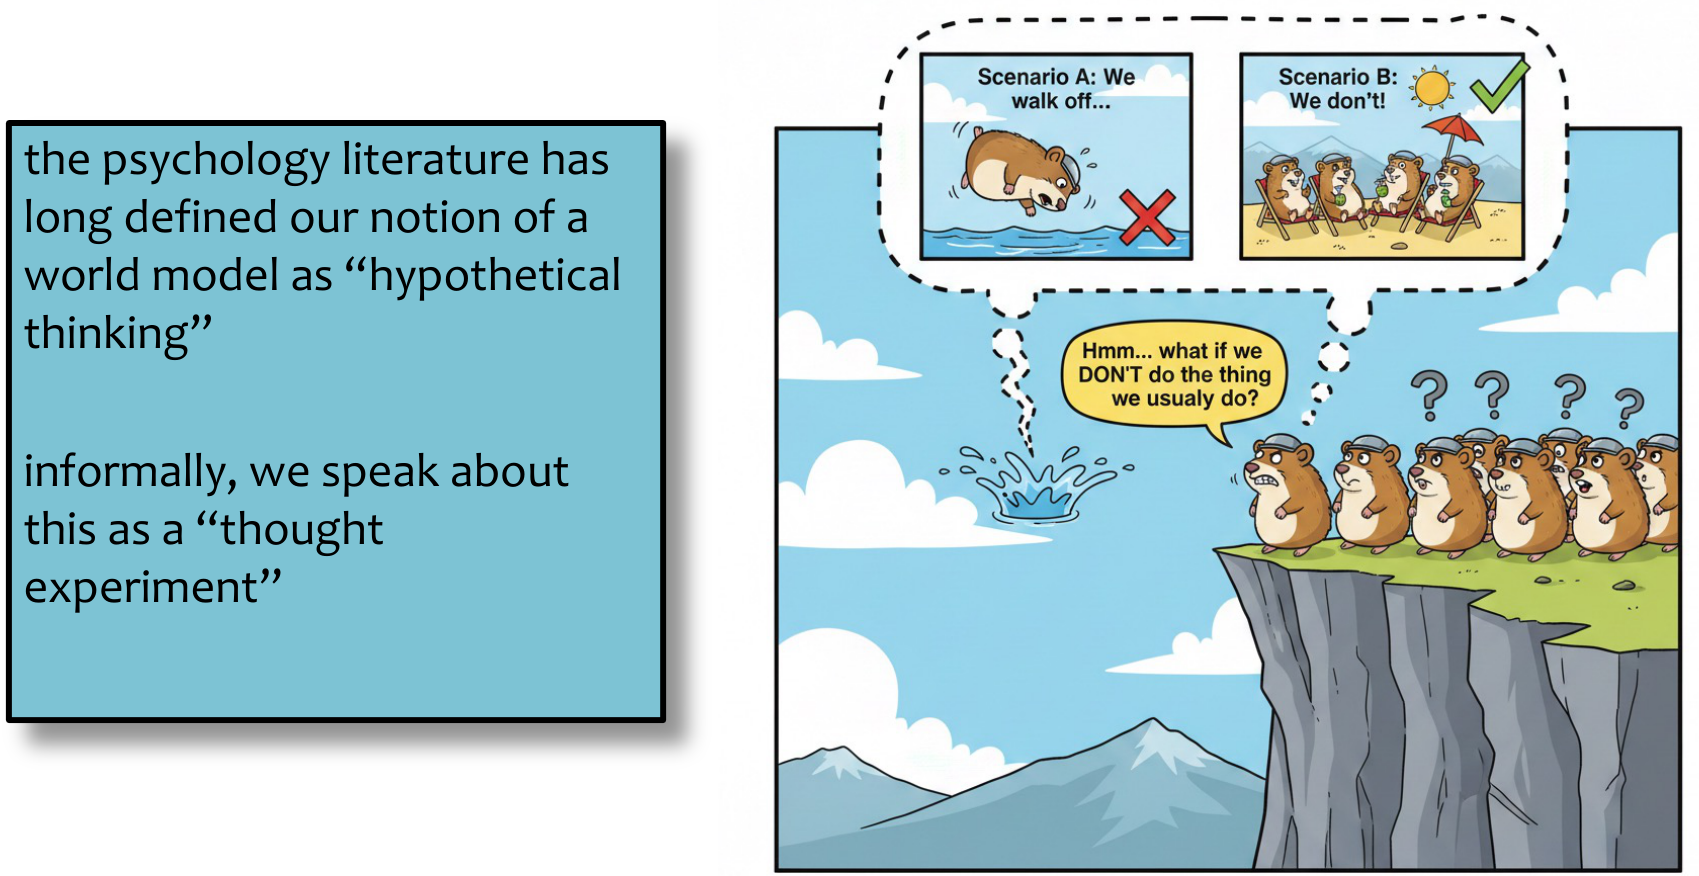
\includegraphics[width=\linewidth,height=0.88\textheight,keepaspectratio]{assets/New-Lecture_World_Models/cmu10423_lecture26_world_models_slide05.png}\\[0.32em]
  {\scriptsize CMU 10-423, Lecture 26.}
\end{frame}

\begin{frame}{World Models: Motivation}
  \begin{itemize}\itemsep0.28em
    \item[\textcolor{red}{$\blacktriangleright$}] Humans develop a mental model of the world based on what they are able to perceive with their limited senses. Our decisions and actions are based on this internal model.    
    \item[\textcolor{red}{$\blacktriangleright$}] Train a generative world model in an unsupervised way to learn a compact spatio-temporal representation of the environment.
    \item[\textcolor{red}{$\blacktriangleright$}] Use features from the world model to train a simple policy (agent) to solve the required task.
  \end{itemize}
\end{frame}

\begin{frame}{World Models: Definition}
  \begin{center}
  \begin{tikzpicture}
    \node[fill=cyan !25, rounded corners=3pt, inner sep=8pt, align=left, drop shadow] (box) {
        \begin{minipage}{0.93\linewidth}
          \textbf{Definition:} \textit{A world model} takes a previous world state $s$ and an action $a$, and samples (or predicts) the next world state $s'$ through a distribution (or function):\\[0.6em]
          \centering
          $s' \sim p(s' \mid s, a)$
        \end{minipage}
    };
  \end{tikzpicture}
  \end{center}
\end{frame}

\begin{frame}{World Models: Definition}
    \textbf{Question:} What does a world state hold?\\[0.4em]

    \textbf{Answer:} It depends on what you're trying to model. Consider the contrast of:
    \begin{itemize}\itemsep0.24em
      \item [A)] All geopolitical entities, their leaders, and decisions they make
      \item [B)] Physical interactions in a 3D world
    \end{itemize}
  \end{frame}

\begin{frame}{World Models: Definition}
  \begin{itemize}
    \item A \textbf{world model} is a learned map that summarizes experience so we can predict (or sample) \textbf{what happens next} and sometimes \textbf{counterfactuals}: ``if I had pushed left \ldots''
    \item An \textbf{agent} chooses actions $a_t$ and receives observations $o_t$ and rewards $r_t$. Planning and learning are easier if we can \textbf{imagine} plausible futures without acting in the real environment.
    \item Core tension: predict \textbf{everything in pixels} (high-dimensional, noisy) vs.\ predict in a \textbf{compact latent space} (lose detail but gain stability and generalization).
  \end{itemize}
\end{frame}
\begin{frame}{How could we use a World Model (WM)?}
  \begin{enumerate}
    \item Generate (simulated) training data for robotics
    \item Generate (simulated) training data for autonomous driving
    \item Create interactive worlds (aka.\ computer games) through prompting
    \item Enable automatic generation / editing / refinement of 3D animation or graphics
    \item Allow a thinking model to hypothesize about physical interactions in the real world
    \item Enable faster creation of environments for virtual reality or augmented reality
  \end{enumerate}
\end{frame}
% \begin{frame}[plain]
%   \centering
%   \vspace{0.1em}
%   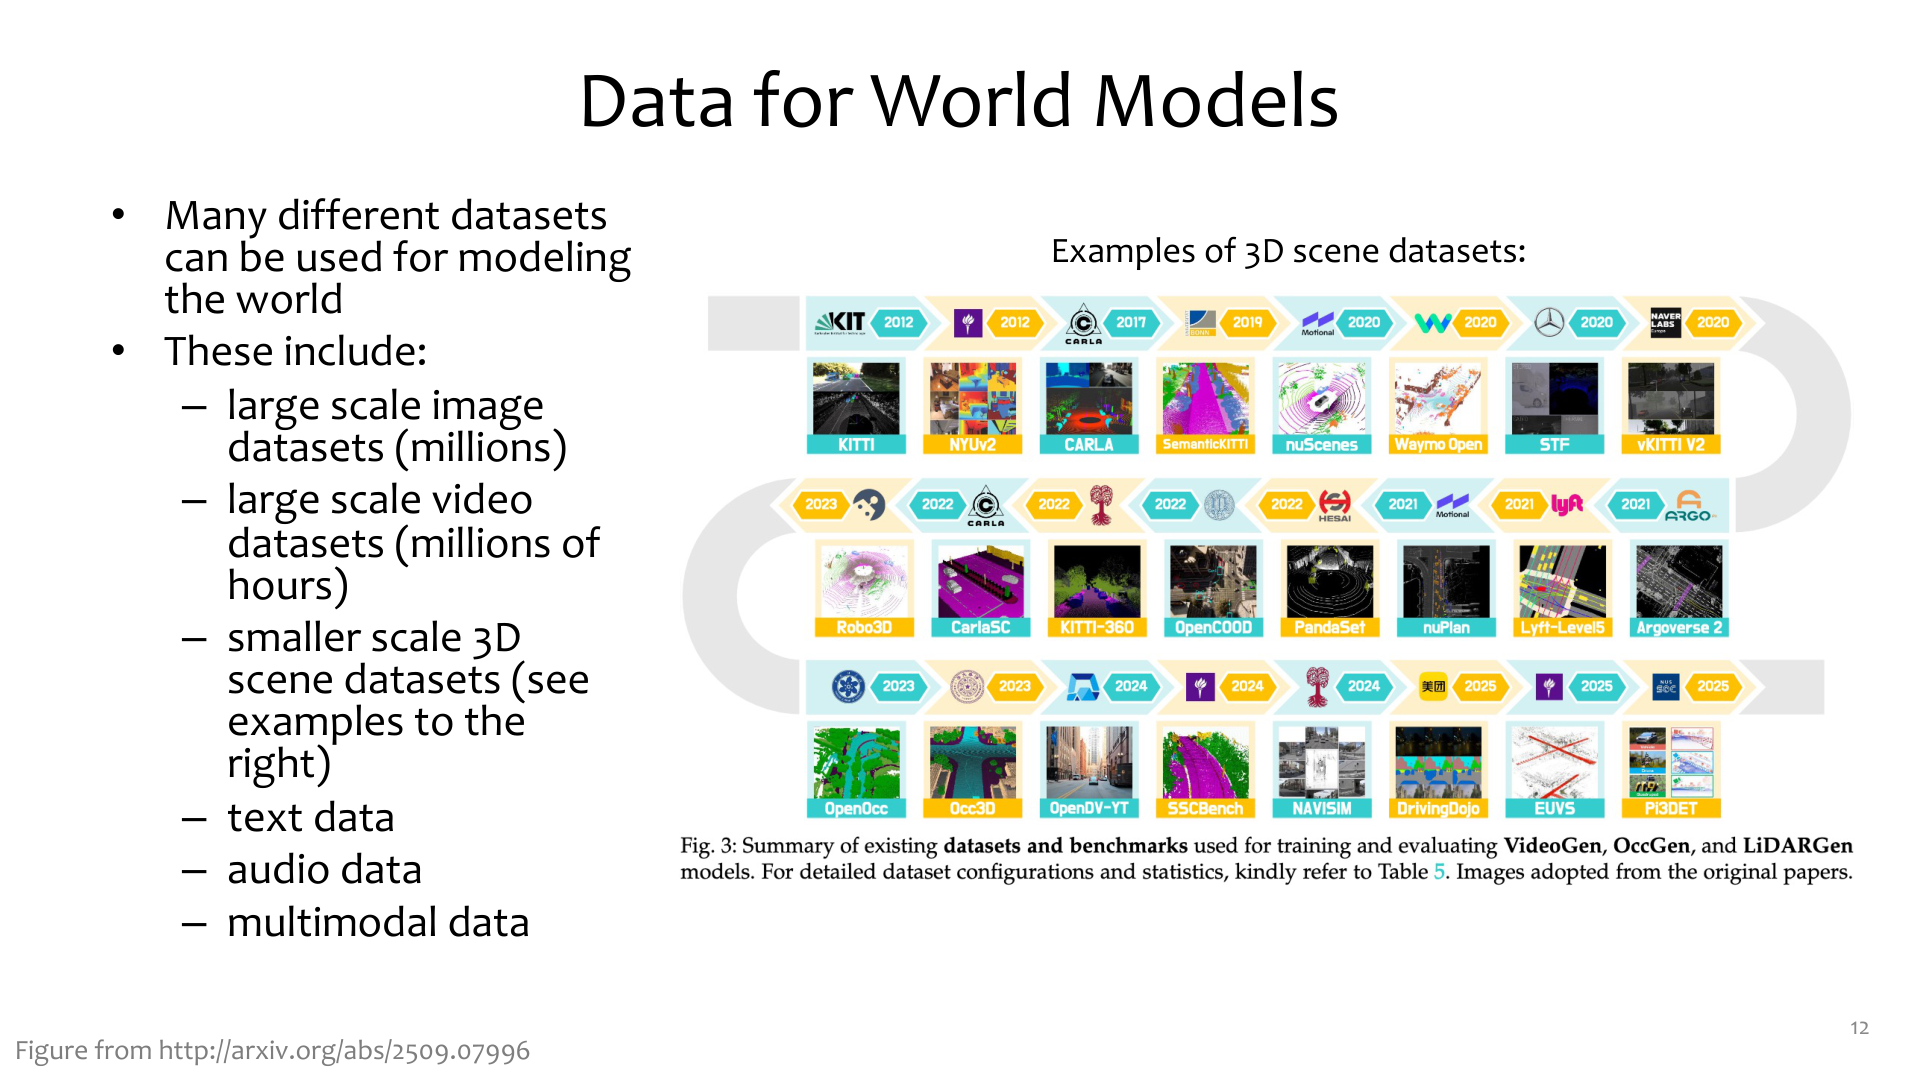
\includegraphics[width=\linewidth,height=0.88\textheight,keepaspectratio]{assets/New-Lecture_World_Models/cmu10423_lecture26_world_models_slide08.png}\\[0.32em]
%   {\scriptsize Same deck --- slide 8 (data modalities: image/video/3D/text/audio/multimodal).}
% \end{frame}

% \begin{frame}[plain]
%   \centering
%   \vspace{0.1em}
%   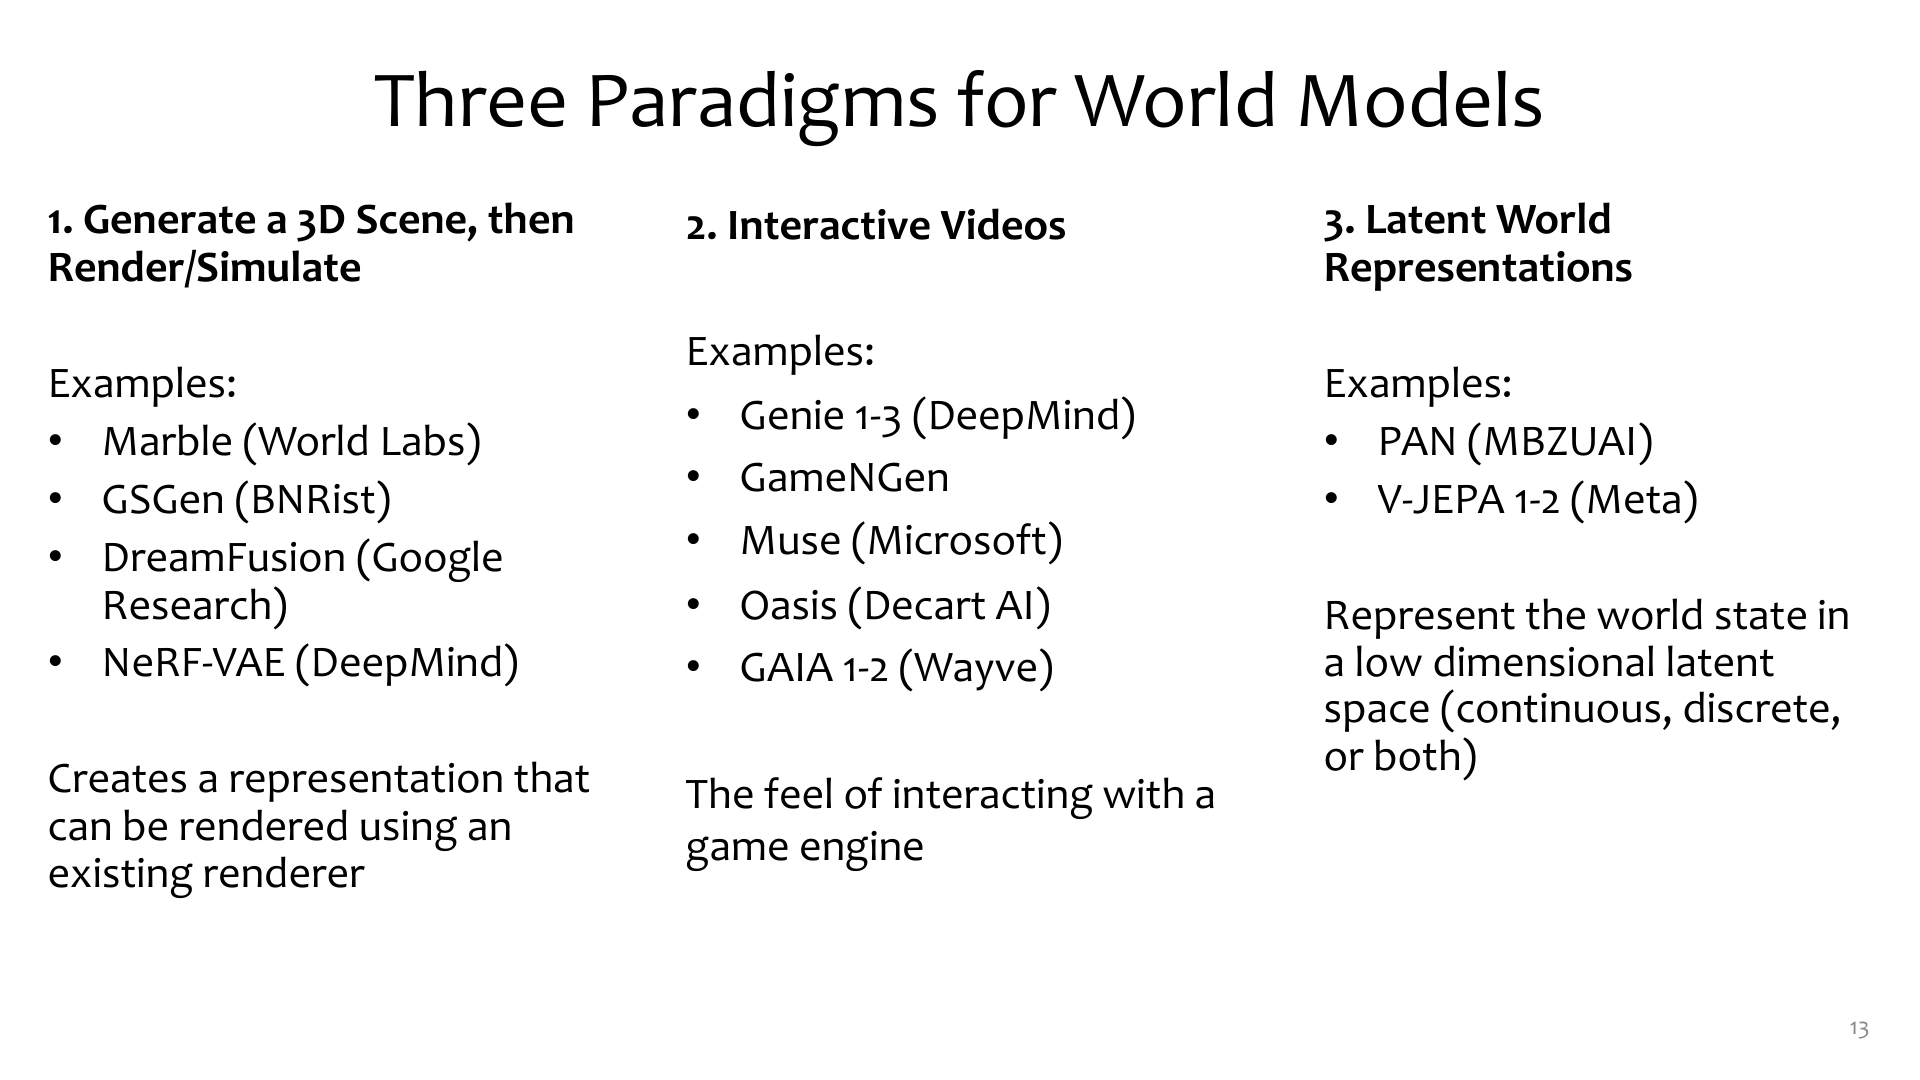
\includegraphics[width=\linewidth,height=0.88\textheight,keepaspectratio]{assets/New-Lecture_World_Models/cmu10423_lecture26_world_models_slide09.png}\\[0.32em]
%   {\scriptsize Same deck --- slide 9 (three paradigms: 3D scene+render; interactive video; latent representations).}
% \end{frame}
\begin{frame}{Some paradigms of World Models}
  \centering
  \vspace{0.1em}
  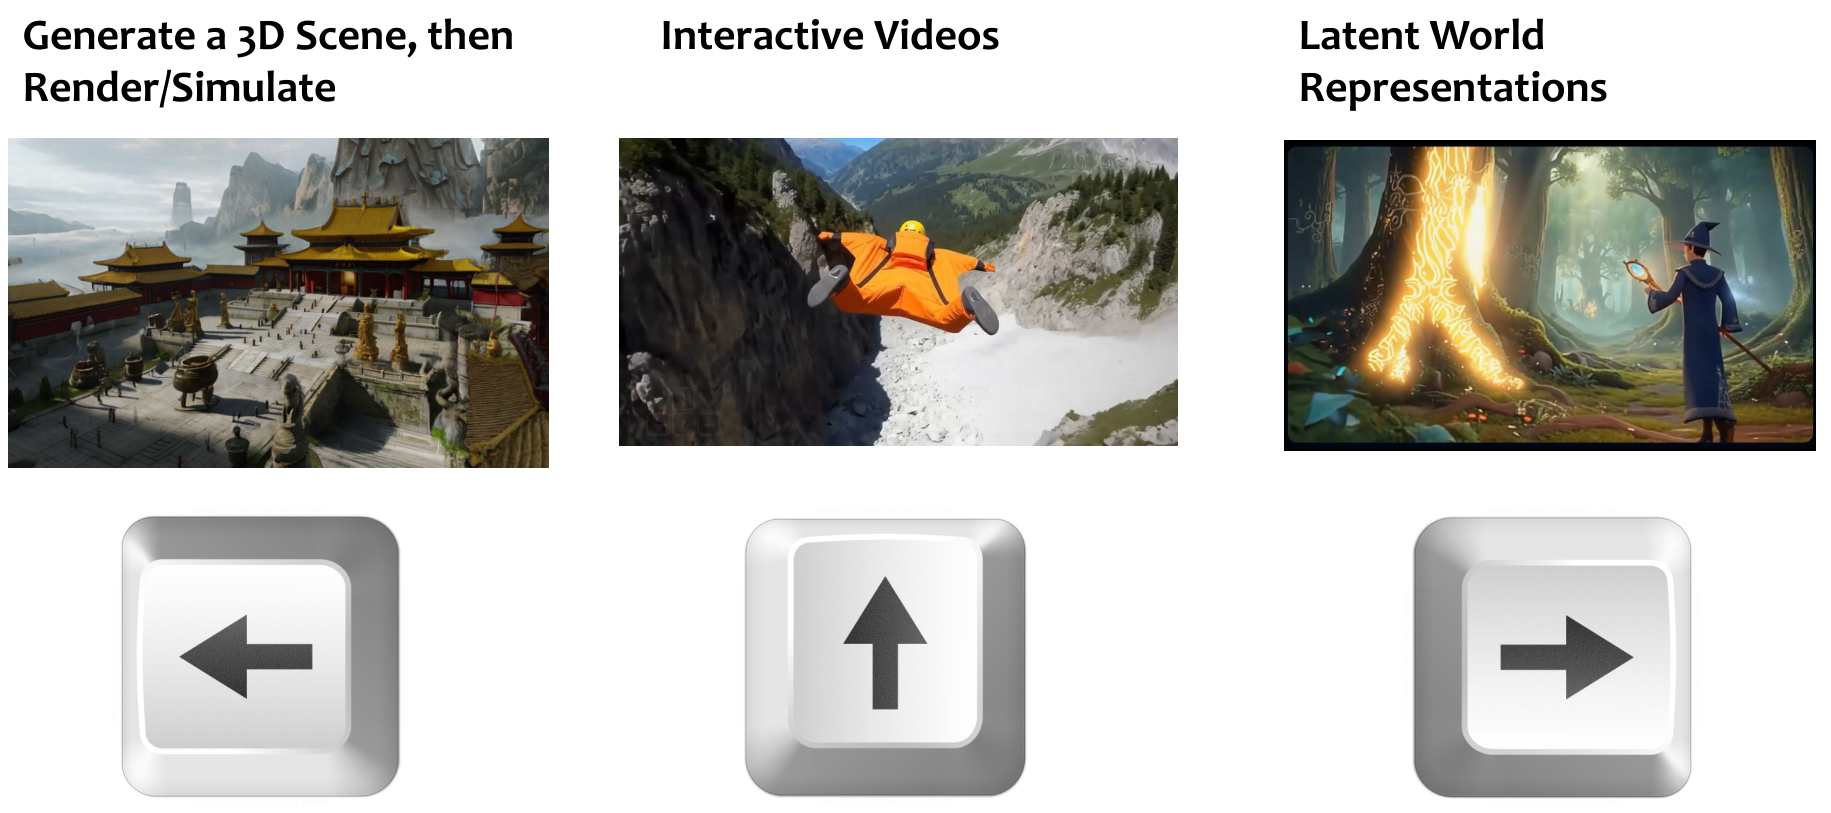
\includegraphics[width=\linewidth,height=0.88\textheight,keepaspectratio]{assets/New-Lecture_World_Models/cmu10423_lecture26_world_models_slide10.png}\\[0.32em]
  {\scriptsize CMU 10-423, Lecture 26.}
\end{frame}

\begin{frame}{Some paradigms of World Models}
  \centering
  \vspace{0.1em}
  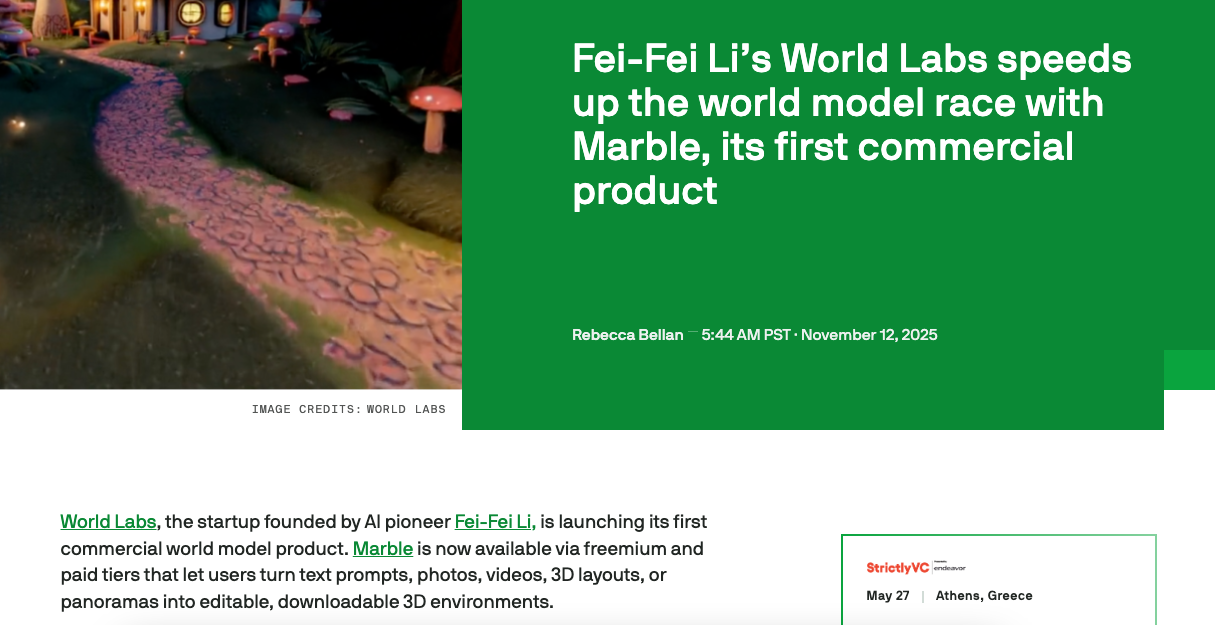
\includegraphics[width=\linewidth,height=0.88\textheight,keepaspectratio]{assets/New-Lecture_World_Models/world_labs.png}\\[0.32em]
  {\scriptsize World Labs.}
\end{frame}
